\begin{figure*}
    \begin{subfig}[t]{.25\textwidth}
    \centering
    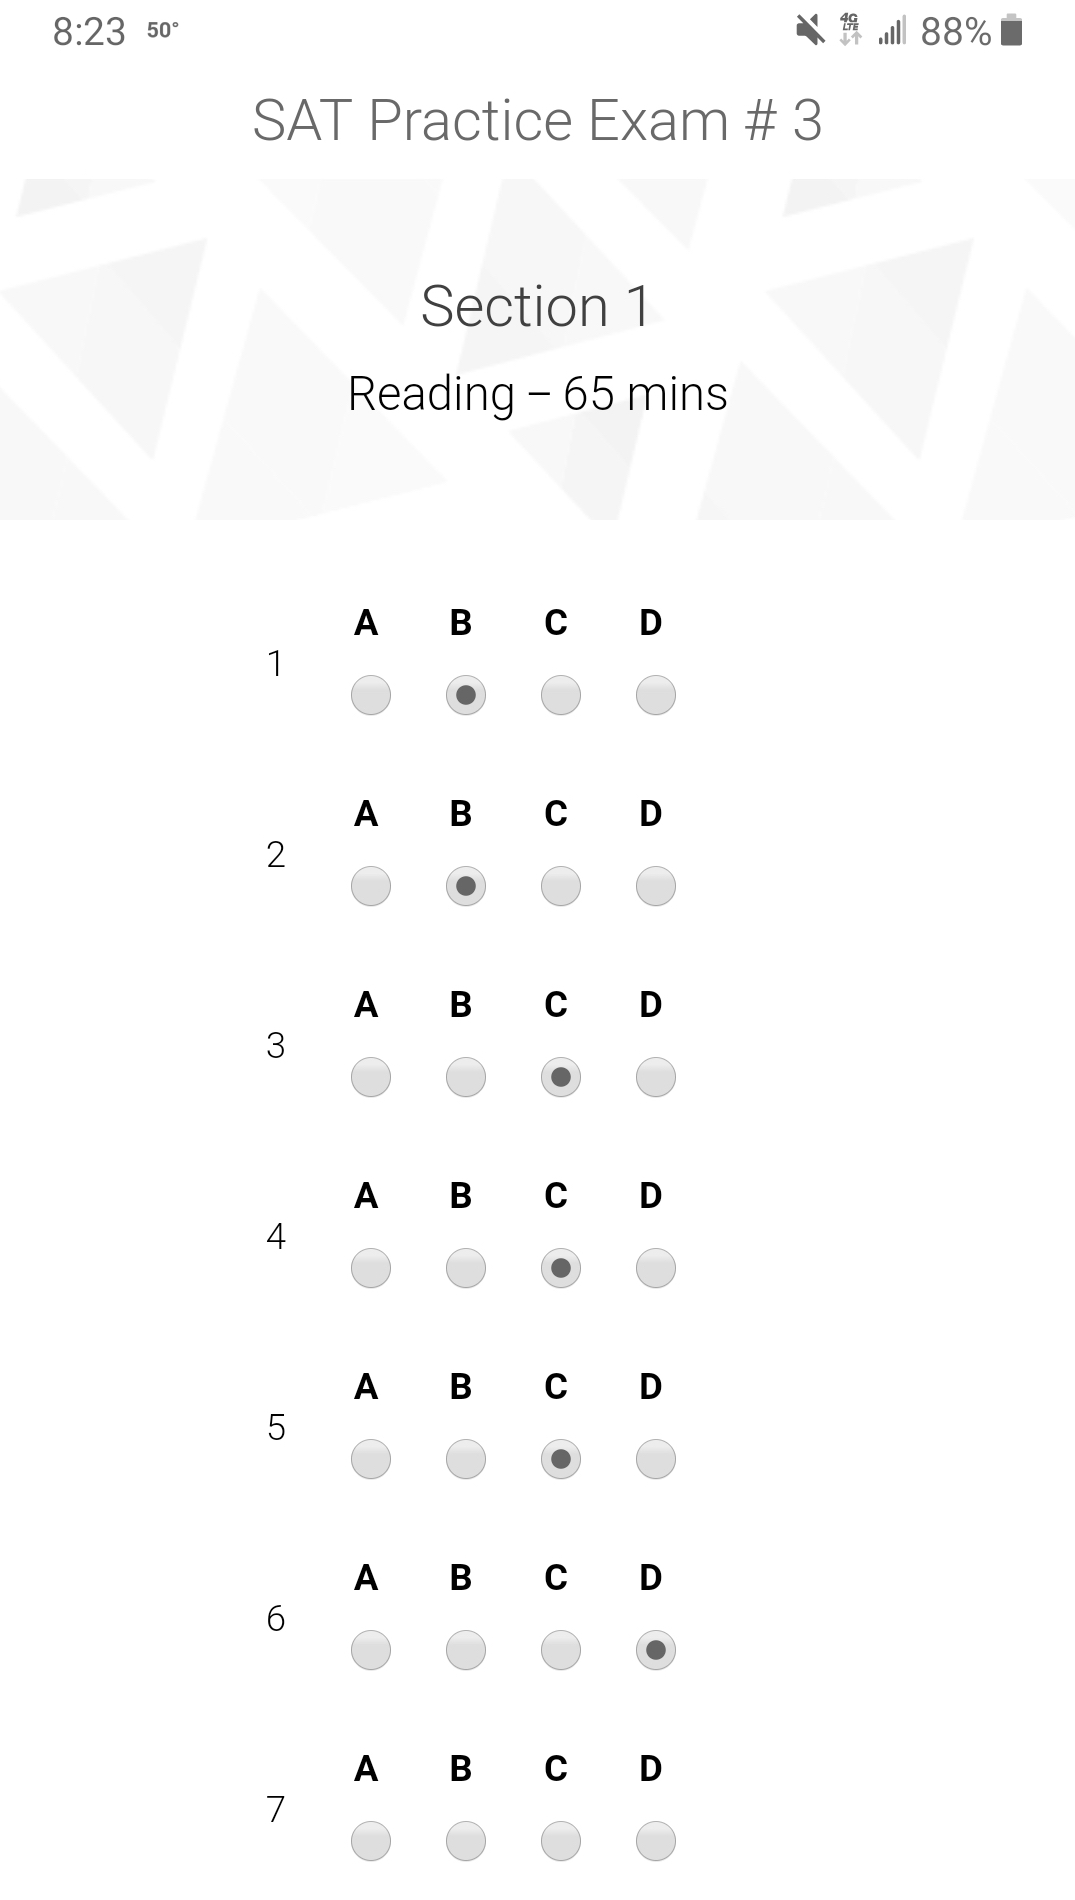
\includegraphics[width=.25\textwidth]{figs/images/ss1.jpg}
    \caption{\ourProgram web interface for test answer input.}
    \label{fig:ss1}
    \end{subfig} \hspace{0.02\textwidth}
    
    \begin{subfig}[t]{.25\textwidth}
    \centering
    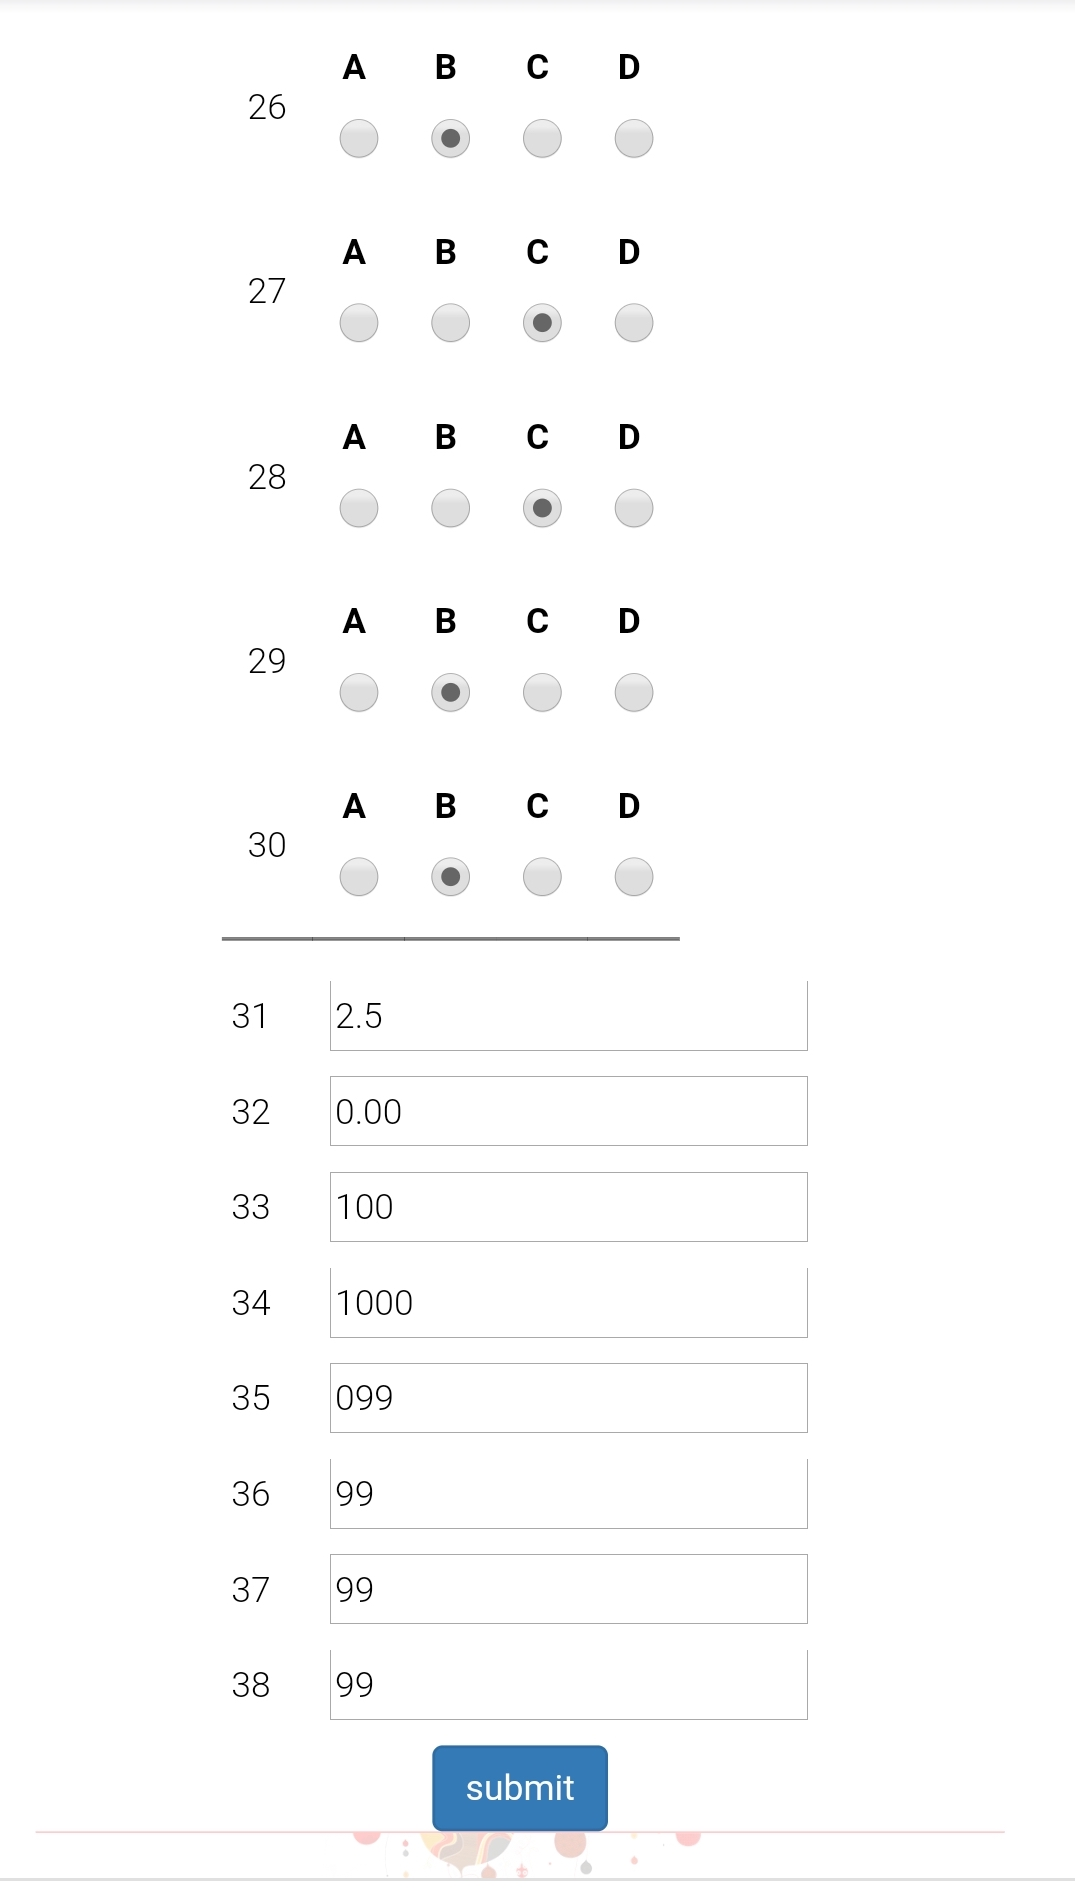
\includegraphics[width=.25\textwidth]{figs/images/ss2.jpg}
    \caption{A student's answer page at the last Math section of the test.}
    \label{fig:ss2}
    \end{subfig} \hspace{0.02\textwidth}
    
    \begin{subfig}[t]{.25\textwidth}
    \centering
    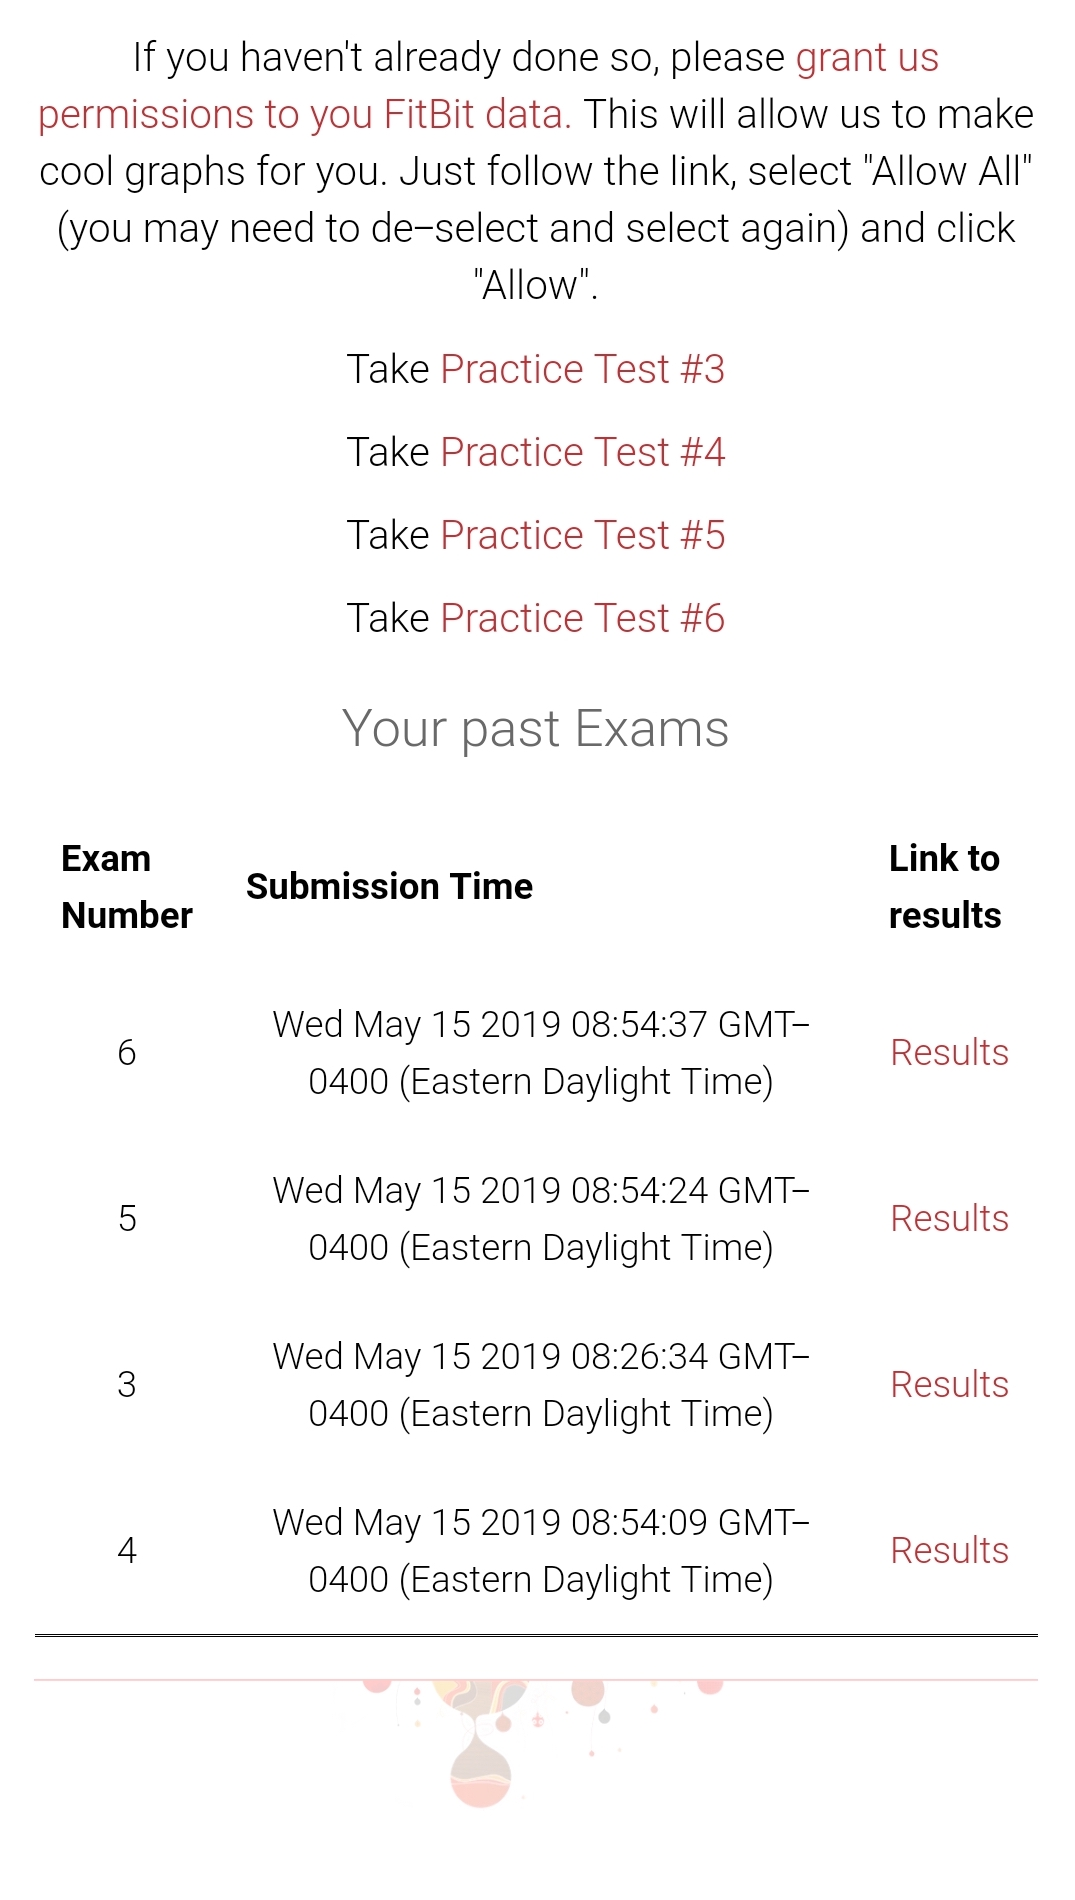
\includegraphics[width=.25\textwidth]{figs/images/ss3.jpg}
    \caption{The page where availability of results are shown.}
    \label{fig:ss3}
    \end{subfig} \hspace{0.02\textwidth}
    
    \begin{subfig}[t]{.25\textwidth}
    \centering
    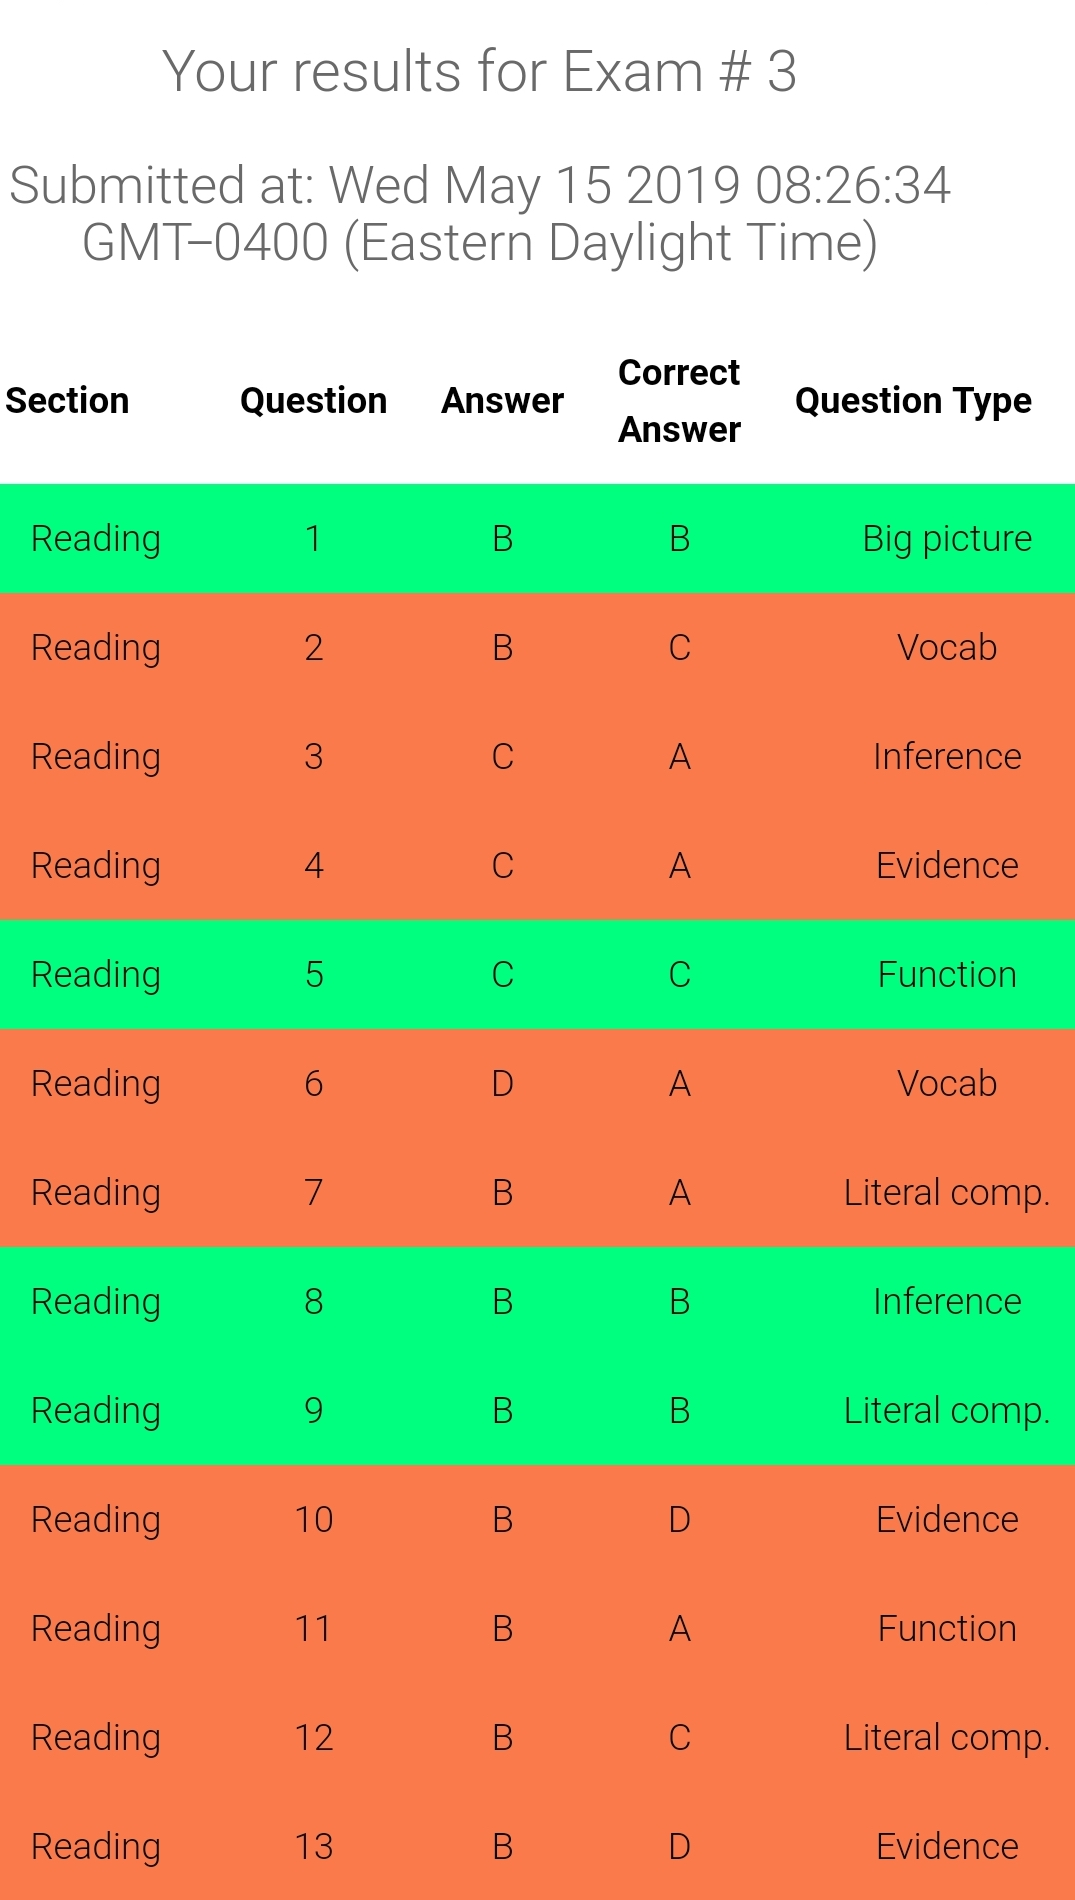
\includegraphics[width=.25\textwidth]{figs/images/ss4.jpg}
    \caption{A student's result page with correct and incorrect answers.}
    \label{fig:ss4}
    \end{subfig}
    
    \caption{EXAMPLE OF HOW FOUR SCREENSHOTS CAN BE LAID OUT NEXT TO EACH OTHER. @SAMMI YOU CAN PUT M4M STUFF HERE.}
    ~\label{fig:screenshots}
\end{figure*}

